
\subsection{流域水治理的分析框架}

% 根据我们的定义,人类活动主导下的人-水关系是社会-水文二元循环中由人类主导的决策模式
% 而水治理(Water Governance)是指影响水使用和管理的政治、社会、经济、和行政系统相互作用的全部过程,本质上是关于“谁获得水,何时获得水,如何获得水”(``who gets water, when and how'')。
联合国开发计划署(UNDP)也提出\cite{undpwatergovernancefacility2016},水治理决定了与水有关的三个核心方面:“什么时候有多少水用?”、“水如何为人类福祉提供不同的生态系统服务?”,以及“谁能平等有效地用水?”——简而言之:有多少水用?怎么用?怎么分?
为此,本章研究将水治理的三个核心方面(“多少水”、“怎么用”和“怎么分”)各自选择指标进行量化,通过对它们进行同等加权,得到综合水治理指数(Integrated Water Governance Index, IWGI)以识别水治理的稳态变化(见图\ref{ch4:fig:framework}~B)。
然后,通过将该指数应用在黄河这个典型的人类活动主导的流域,利用突变点检测的方法分析了$1965\sim2013$年间IWGI的变化,展示该IWGI如何有助于检测和描述复杂的水治理稳态变迁。
最后,在综合分析了水资源供需、经济发展、环境变迁,以及制度变化后,我们解释了黄河流域水治理稳态变化的主要驱动因素,并总结提出了一个过渡模式,为人类活动主导大河流域面临的治理挑战提供了一个实践指南。

\begin{figure}[!ht]
\centering
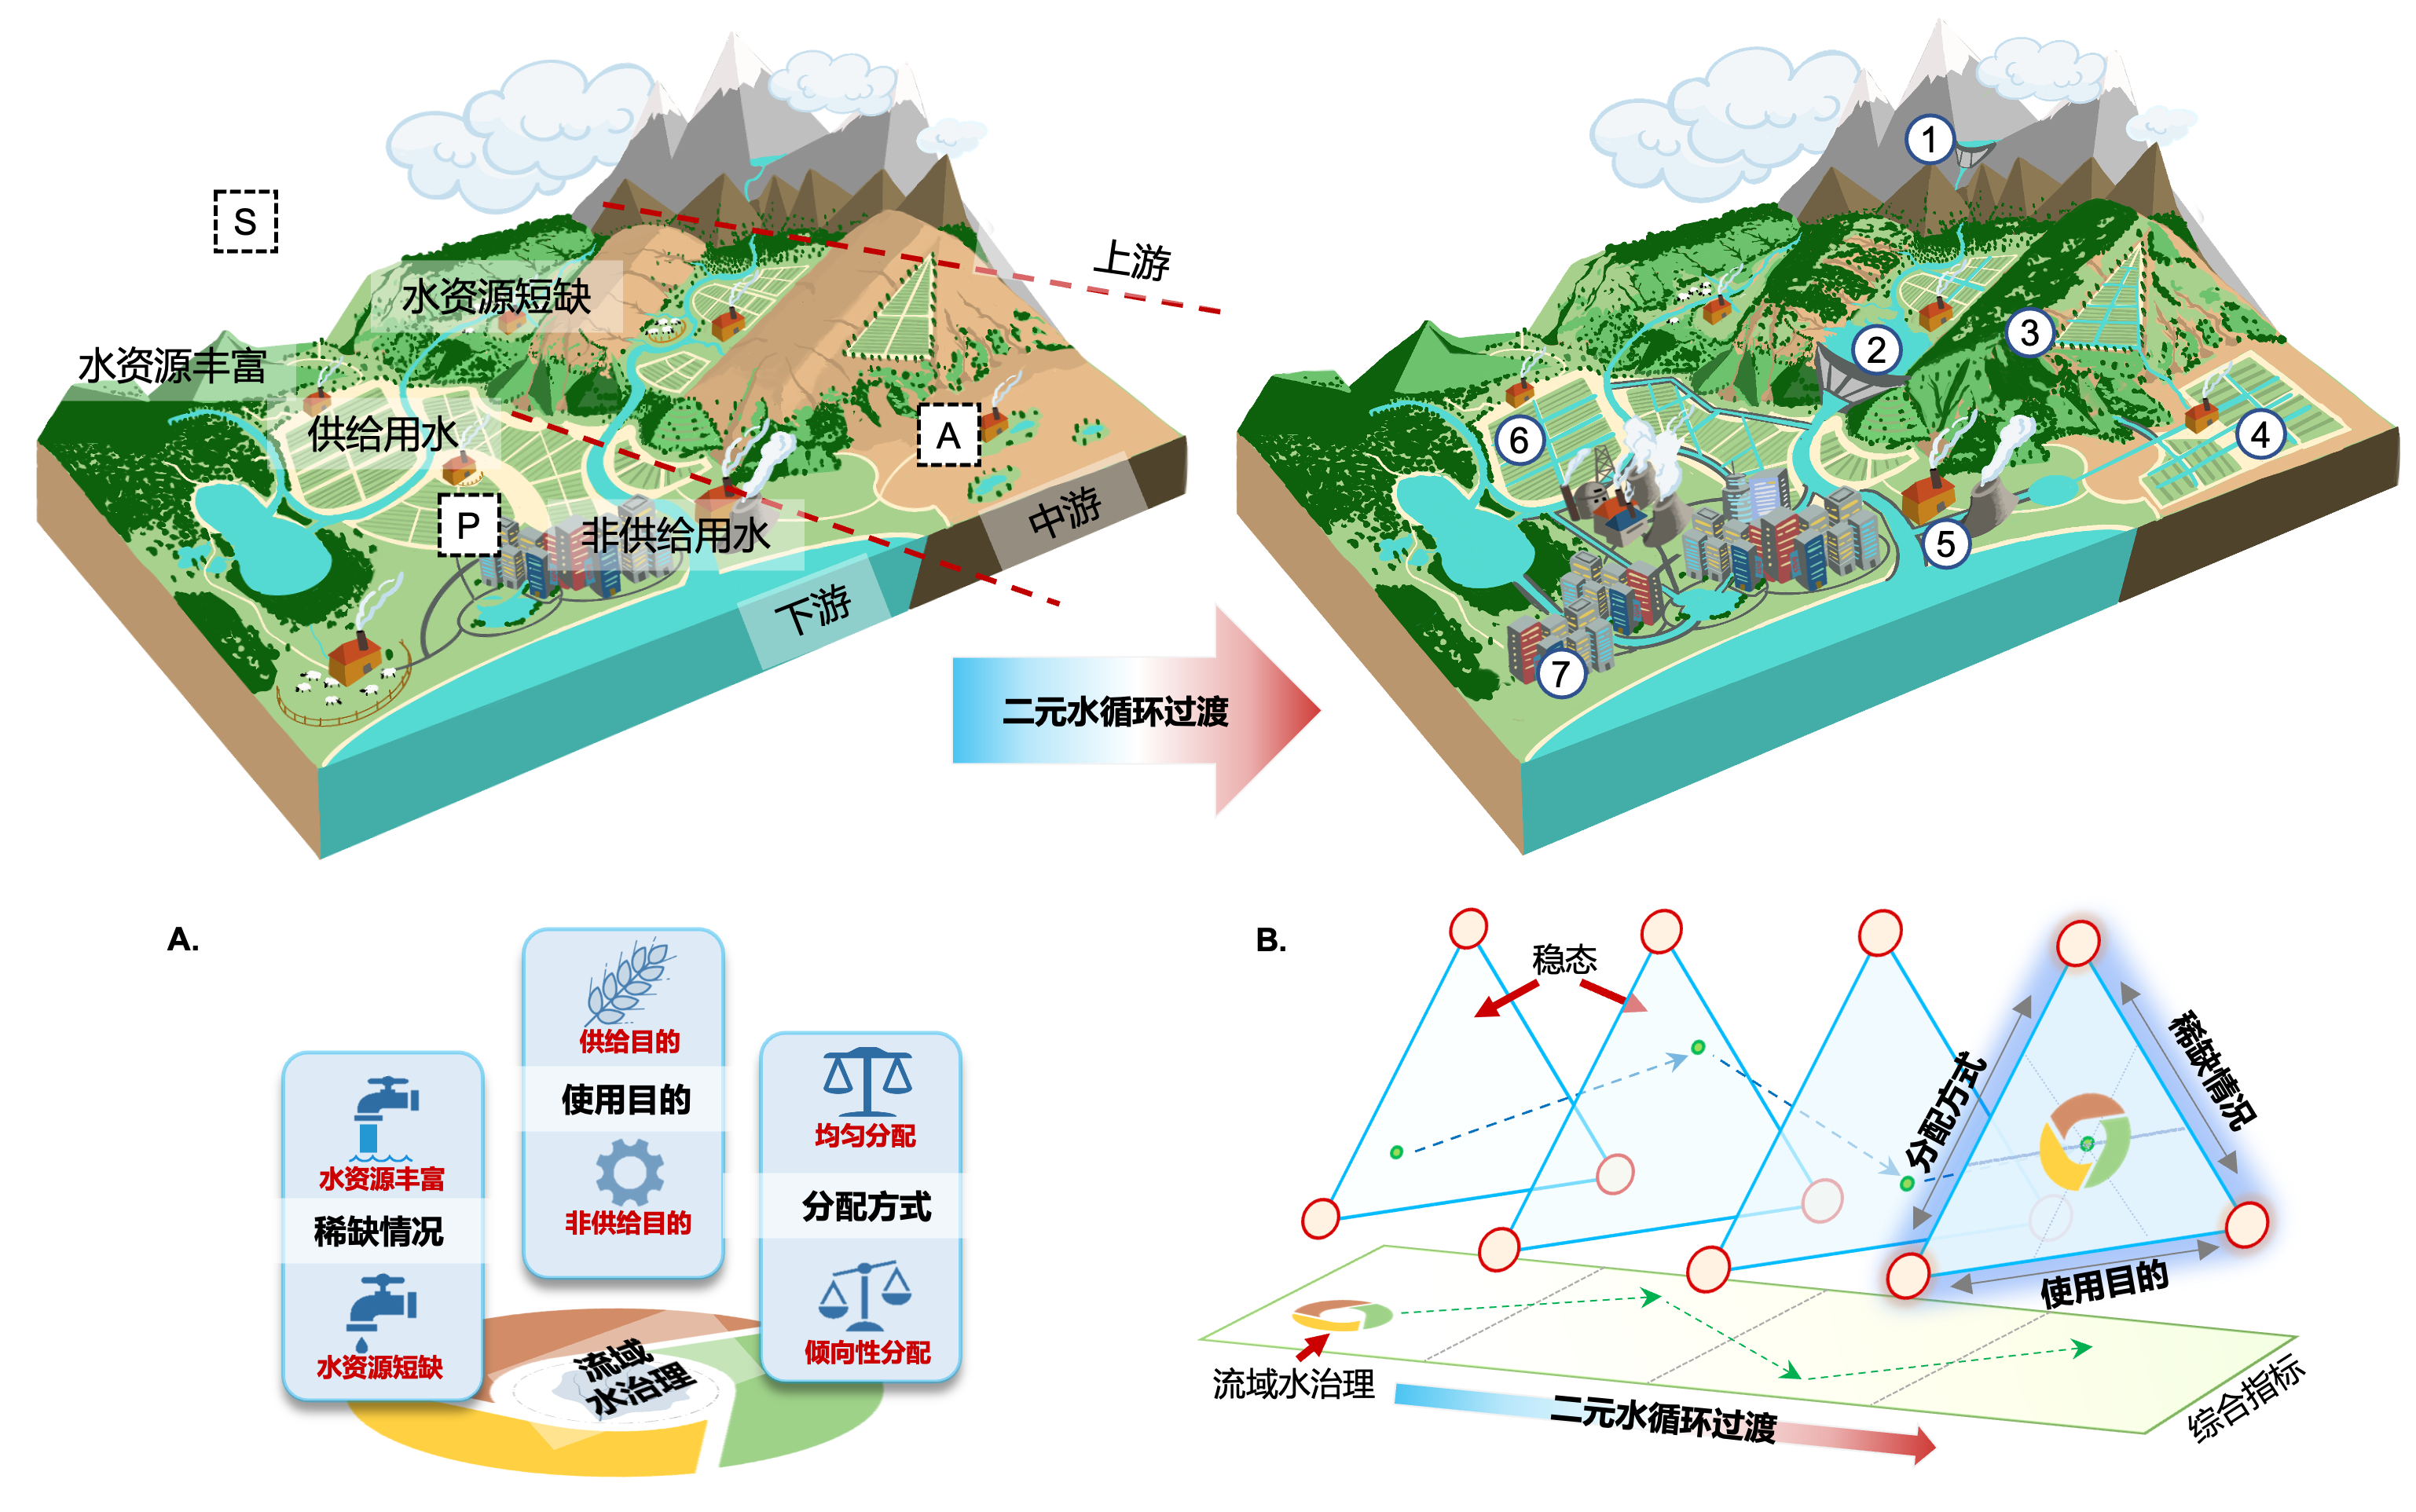
\includegraphics[width=\textwidth]{img/ch4/ch4_framework.png}
\caption[定量识别流域水治理转变的分析框架]{
    利用综合水治理指数(IWGI)识别水自然-社会二元循环过渡时期中的水治理机制,可以从“有多少水用”(S)、“怎么用”(P)和“怎么分”(A)这三个主要方面切入(\textbf{A.})。水治理的这三个方面会随着人类活动主导社会-水文循环而变化。例如,水库建设(1)可以缓解局地水资源压力;能源和工业增长(2)、集约化灌溉农业的发展(3)会改变水的利用方式;输水系统(4)控制了流域系统的水分配。IWGI方法结合三个方面的相应指标,因此其突变可以指示水治理的稳态转换(\textbf{B.})。}\label{ch4:fig:framework}
\end{figure}

\subsection{黄河子区域划分}\label{ch4:sec:region}

为便于研究的计算需要,本章参考前人研究和黄河水利委员会的标准将黄河流域划分为四个区域\cite{shuilibuhuangheshuiliweiyuanhui,wang2019c,wang2016e},以四个重要的控制水文站反映各区域的径流变化,各区域特点鲜明,便于后文对水资源治理的变化原因进行分析:

\textbf{黄河源区(SR):}(唐乃亥站)人口稀少,经济欠发达,主要生态功能是水源涵养,黄河超$50\%$的天然径流来自这里。
\textbf{黄河上游(SR):}(头道拐站)人均灌溉土地面积最高的区域,大量引黄河水发展灌溉农业,但灌溉效率相对较低。
\textbf{黄河中游(MR):}(花园口站)黄河在此流经著名的富沙区——黄土高原,作为土壤侵蚀风险最高的地区,是黄河产沙最多的地区,近三十年对“退耕还林”生态工程显著改变了这里的土地利用覆被。
\textbf{黄河下游(LR):}(利津站)人口密集,传统的农业发达地区,也曾是最大的黄河水资源使用地区。然而随着产业升级和节水工程的持续,尽管仍是总用水最多的地区,农业用水的比重不断下降。


% % 补充图片1:研究区示意图
% \begin{figure}[hbtp!]
% \centering
% 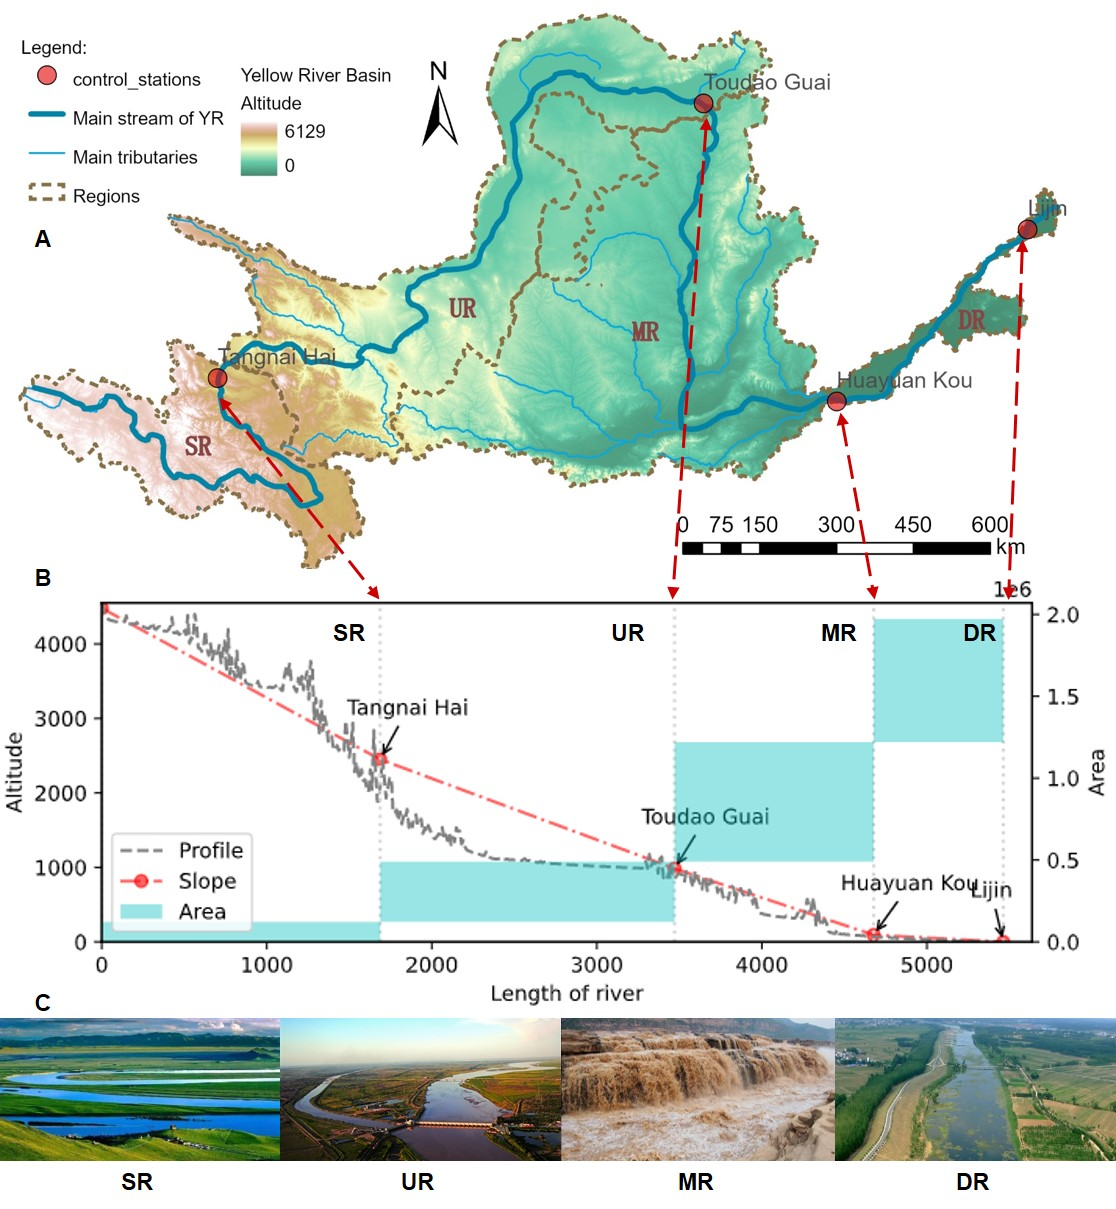
\includegraphics[width=\textwidth]{img/ch4/s1_study_area.jpg}
% \caption[黄河流域子区域划分]{黄河流域子区域划分。
%     \textbf{A.}黄河流域划分示意图(SR:源区,UR:上游,MR:中游,DR:下游);
%     \textbf{B.}黄河主河道剖面图,四个水文观测站分别控制SR、UR、MR和DR;
%     \textbf{C.}黄河流域不同地区的典型景观。}\label{fig:YRB}
% \end{figure}

\subsection{水资源治理综合指数}

% 将三者合一起,即:
如本章前文介绍以及框架图~\ref{ch4:fig:framework}所示,我们定义的水资源治理综合指数(IWGI)应结合水治理的三个方面(“多少水(S)”、“怎么用(P)”和“怎么分(A)”)。
由于每个指标维度都有升高和降低两个方向,在整合指标前应假设随着人类活动主导社会-水文循环的进程,三者在其中某个方向对齐:

\begin{equation}
    Transformation \propto S*P*A
\end{equation}

接下来为三个方面选择了一个指标($I_x$, $x=S$, $P$,或$A$,分别对应“多少水(S)”、“怎么用(P)”和“怎么分(A)”,来有效地量化这些方面,并将上式转化为自然对数,便于计算各指标对综合指数变化的贡献:

\begin{equation}
    Transformation \propto \ln(I_S) + \ln(I_P) + \ln(I_A)
\end{equation}

那么,综合水治理指数(IWGI)是标准化指标$I'_x$的平均值:
\begin{equation}
    IWGI = (I'_S + I'_P + I'_A) / 3
\end{equation}

其中:
\begin{equation}
    I'_x = (I_x - I_{x, \min}) / (I_{x, \max} - I_{x, \min})
\end{equation}

对三个方面各自的指标选取如下文所述。

\subsubsection*{“有多少水(A)”}

“有多少水用”不仅取决于气候能提供多少水资源(而且在许多地区日益稀缺和不确定性),还取决于灌溉和工业等经济活动的需求(日益无法被满足),更可以被水库蓄水、跨流域调水等工程所人为改变\cite{qin2019,wada2014,huang2021}。
本章研究采用Qin等人(2019)提出的稀缺性-韧性-易变性(SFV)水稀缺指数来评价“有多少水”的问题\cite{qin2019}。
这一指标考虑了管理措施(如水库的建设)和用水结构变化(有些用水方式如能源用水是难以被短期替代的),对水资源短缺情况做出评估。
此外,SFV指数还考虑了水资源的灵活性和易变性(例如气候差异带来的降水波动),从发展的角度关注水资源的动态,是衡量水资源压力\cite{qin2019}时间变化的有效指标。
整个黄河流域的水分胁迫指标$I_S$为本章划分的四个二级区域$i$——源区(SR)、上区(UR)、中游(MR)、和下游(DR)指数$SFV_{i}$的平均值:

\begin{equation}
    I_S = \frac{1}{4} * \sum_{i=1}^4 SFV_{i}
\end{equation}

其中$SFV_i$为区域$i$的SFV指数$SFV_i$,SFV结合了以下三个指标:

首先,对于稀缺性(Scarcity, S),$A_{i, j}$为区域$i$在第$j$年的耗水量占多年平均径流量的比例(本研将为黄河流域划分为四个子区域,见\ref{ch4:sec:region}\nameref{ch4:sec:region}):

\begin{equation}
    A_{i, j} = \frac{WU_{i,j}}{R_{i, avg}}
\end{equation}

% TODO 完整的不灵活用水分类?
其次,对于灵活性(Flexibility, F),$F_{i, j}$是第$i$年和第$j$区域的不灵活用水$WU_{inflexible}$(例如能源行业冷却用水或人类和牲畜)占平均多年径流量的比例:

\begin{equation}
    F_{i, j} = \frac{WU_{i, j, inflexible}}{R_{i, avg}}
\end{equation}

最后,易变性(Variability, V)还考虑了水库容量和蓄水对自然径流波动的积极影响:
\begin{gather}
    C_i = C1_i * (1 - C2_i) \\
    C1_{i, j} = \frac{R_{i, std}}{R_{i, avg}} \\
    C2_{i} = \frac{RC_{i}}{R_{i, avg}}, \ if RC < R_{i, avg} \\
    C2_{i} = 1, \ if RC >= R_{i, avg}
\end{gather}

上式中,$R_{i, avg}$为$i$区域的平均径流量,$RC_i$为$i$区域水库的总库容,$R_{i, std}$为$i$区域径流量的标准差。

最后,该方法将三个指标(稀缺性S、灵活性F和易变性V)以相同的权重进行归一化后加权计算出$SFV$指标:

\begin{gather}
    V = \frac{A_{normalize} + B_{normalize} + C_{normalize}}{3}\\
    a = \frac{1}{V_{\max} - V_{\min}};\\
    b = \frac{1}{V_{\min} - V_{\max}} * V_{\min}\\
    SFV = a * V + b
\end{gather}


\subsubsection*{“怎么用水(P)”}

“怎么用水”与水能够提供的生态系统服务有关,但目前对文化、调节服务等缺乏成熟统一的评估框架,且受限于数据,本研究仅将用水分为供给用途(例如,日常饮用和食品生产)和非供给用途(例如能源冷却用水)的用水\cite{liu2017,florke2018,jaeger2019}。
本章研究使用非供给服务目的在全部用水量中所占比例(Non-provisioning Share, NPS)作为量化“怎么用水(P)”$I_P$的指标。

\begin{equation}
    NPS = \frac{WU_{pro}}{WU_{pro} + WU_{non-pro}}
\end{equation}

其中($WU_{pro}$)为供给服务用水,包括家庭用水、灌溉用水和牲畜用水;非供给服务的用水($WU_{non-pro}$)包括工业用水和城市服务用水。
% 本章研究将牲畜用水、城乡生活用水和农业用水作为供应用水,因为它们直接服务于生存。其他的是非供应:服务和工业用水,因为它们主要为经济服务。% TODO 完整的供应水分类?

\subsubsection*{“怎么分水(A)”}

最后,“怎么分水”也并非取决于区域的社会经济水平和自然环境背景,流域的水资源分配还会受到流域系统调度的工程(如水库统一调度)、非工程因素(如水资源分配制度)的影响\cite{schmandt2021,speed2013}。
为了描述分配$I_A$,本章研究设计了一个基于熵的分配度量指标,它衡量水分配的均匀程度:

\begin{equation}
    I_A = CEM = \sum_{i=1}^N - \log(p_{i}) * p_{i}
\end{equation}

其中$p_{i}$为区域$i$与整个流域的水量比例,$N=4$。

\subsection{突变点检测}

本章研究采用Pettitt(1979)提出的的突变点检测方法,在不假设数据分布的情况下,对水文时间序列数据的单个变化点进行检测\cite{pettitt1979}。
它测试的原假设$H0$是:变量不存在存在变化趋势差异,备择假设则为存在一个变化趋势点。
数学上,将随机变量序列分为$\mathrm{x}_{1}, \mathrm{x}_{1}, \ldots, x_{t_{0}}$和$x_{t_{0}+1}, x_{t_{0}+2}, \ldots, x_{T}$表示的两段,如果每段都有一个共同的分布函数,即$F_1(x)$、$F_2(x)$和$F_1(x) \neq F_2(x)$,则在$t_0$处确定变化点。

为实现变化点的识别,定义统计指标$U_{t,T}$如下:

\begin{equation}
    U_{t, T} = \sum_{i=1}^t\sum_{j=t+1}^T sgn(X_i - X_j), 1 \leq t < T
\end{equation}

其中:
\begin{equation}
    \operatorname{sgn}(\theta)= \begin{cases}1 & \text { if } \theta>0 \\ 0 & \text { if } \theta=0 \\ -1 & \text { if } \theta<0\end{cases}
\end{equation}

找到最可能的变化点$\tau$,其值满足$K_{\tau} = \max|U_{t, T}|$,与值$K_{\tau}$相关的显著性概率近似计算为:

\begin{equation}
    p=2 \exp \left(\frac{-6 K_{\tau}^{2}}{T^{2}+T^{3}}\right)
\end{equation}

给定某个显著性水平$\alpha$,如果$p < \alpha$,则拒绝原假设并得出结论$x_{\tau}$是水平$\alpha$的显著突变点。

本章研究使用$\alpha = 0.001$作为显著性$p$的阈值,这意味着统计上显著的变化点判断有效的概率大于$99.9\%$。
迭代使用Pettitt算法:反复识别一个突变点从而将时间序列分为该时间点前后两段,并再次分别对两序列进行分析,直到检测到所有显著的突变点。
虽然接下来的结果展示的是阈值$\alpha = 0.001$的结果(识别出两个断点),但是经过我们的敏感性分析,从$0.0005$到$0.05$的阈值范围选取都不影响本研究结果的鲁棒性(参见图\ref{ch4:fig:sensitivity})。

\begin{figure}[htb] % use float package if you want it here
    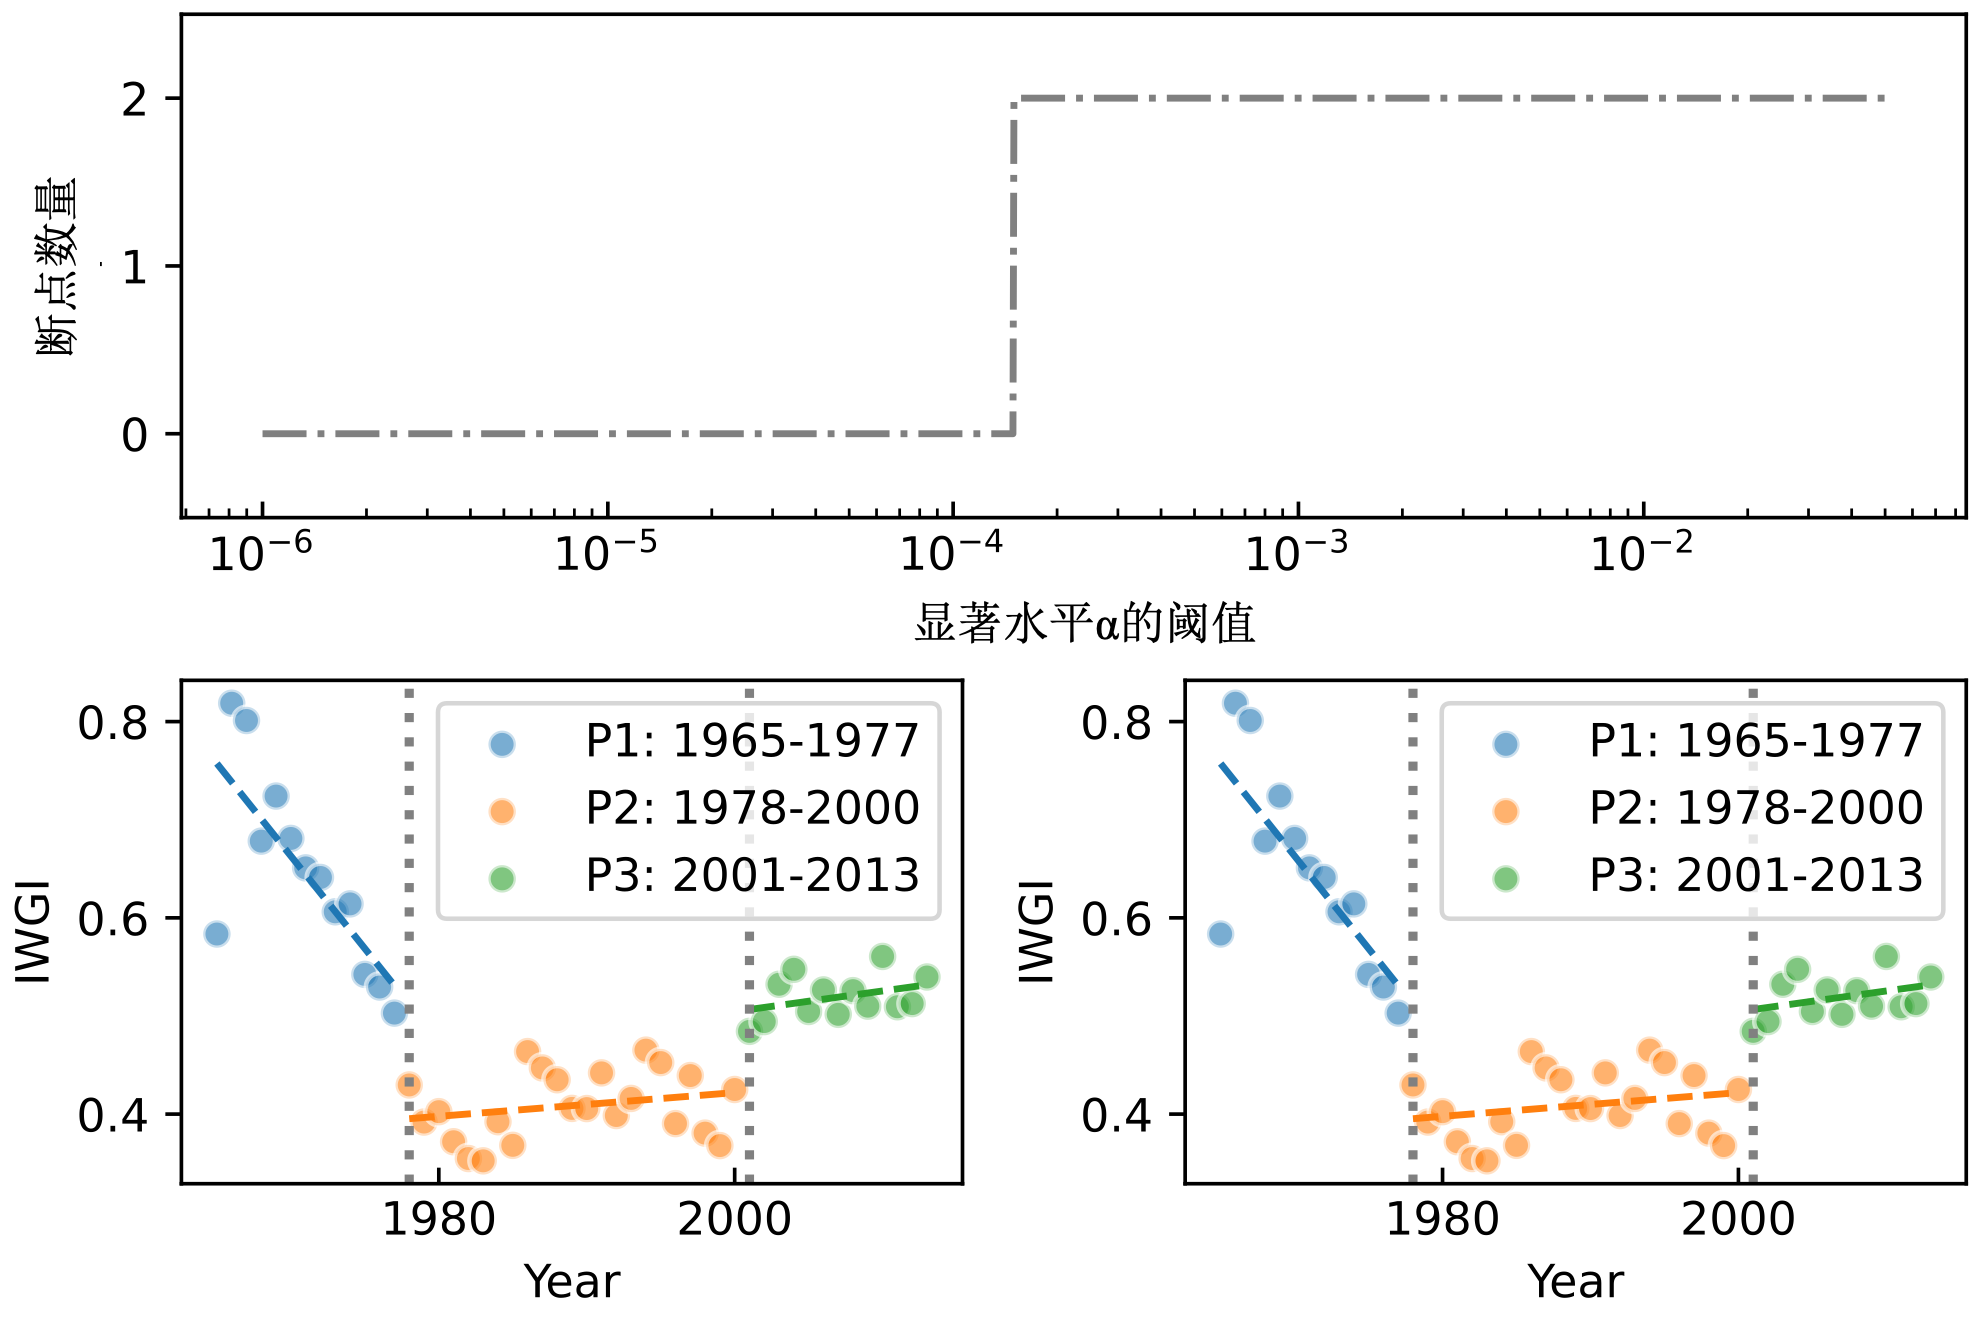
\includegraphics[width=\textwidth]{img/ch4/ch4_sensitivity.png}
    \caption[断点识别中显著性阈值选取的敏感性测试]{断点识别中显著性阈值选取的敏感性测试结果。
    \textbf{A.} 选取不同阈值$\alpha$后识别的突变点个数,所有的方案都识别了两个断点。
    \textbf{B.} 阈值选取为 $\alpha=0.0005$.
    \textbf{C.} 阈值选取为 $\alpha=0.05$.}\label{ch4:fig:sensitivity}
\end{figure}

\subsection{数据来源与处理}
本章研究需要计算诸多指标和子指标,所有使用的数据集都在表\ref{ch4:tab:data_source}中列出,根据原始数据的收集方式,主要包括了统计资料、水文数据、书面文献三类。

% Table generated by Excel2LaTeX from sheet '数据集'
\begin{table}[htbp]
    \centering
    \caption{数据分类与来源}
      \begin{tabularx}{\textwidth}{LLLLL}
      \toprule
      数据集   & 数据类型  & 空间尺度  & 时间尺度  & 数据来源 \\
      \midrule
      行政区水资源利用 & 统计    & 市级行政单元 & $1965-2013$ & Zhou等人2020 \\
      子流域水资源使用 & 统计    & 二级子流域 & $2003-2019$ & 水资源公报 \\
      GDP数据 & 统计    & 省级行政单元 & $1949-2019$ & 万德数据库 \\
      水库数据集 & 水文    & 站点数据  & $1949-2015$ & Wang等人2019 \\
      实测泾流量 & 水文    & 站点数据  & $1949-2019$ & Wang等人2019 \\
      黄河流域相关法律 & 文献    & 流域相关文件 & $1949-2013$ & 黄河流域规划 \\
      黄河水利委员会历史 & 文献    & 流域相关文件 & $1949-2002$ & 黄河水利委员会档案馆 \\
      黄河大事件 & 文献    & 流域相关文件 & $1949-2015$ & 黄河水利委员会档案馆 \\
      \bottomrule
      \end{tabularx}%
    \label{ch4:tab:data_source}%
\end{table}%
  

\subsubsection*{统计资料}
我们使用的GDP数据、人口数据等来自于国家统计局的统计年鉴\url{http://www.stats.gov.cn/tjsj/ndsj/2019/indexeh.htm}。
水资源相关数据来源于第二次国家水资源调查\cite{zhou2020}和水文统计年鉴\url{http://www.yrcc.gov.cn/other/hhgb/}。
水资源利用数据集由Zhou等人于2020年\cite{zhou2020}发布,该数据集记录了各地级市不同用水部门的水资源使用情况。
第二次国家水资源调查是由国家发展和改革委员会以及水利部牵头启动的数据统计项目(详见\url{http://www.mwr.gov.cn/english/publs/}),所有数据已使用相同的标准匹配到2013年的行政区划。
该数据涵盖了四个大类的用水情况:农业(IRR)、工业(IND)、城市(URB)和农村(RUR)用水(详见Zhou等人,2020\cite{zhou2020})。
尽管每个用水部门的分类在县尺度上都存在一定程度上的数据不确定性,但由于相关部门已使用过水平衡方法对统计信息进行了校正,因此该数据足以用于本研究中使用的区域尺度研究。

\subsubsection*{水文数据}
水库名录数据集由Wang等人\cite{wang2019c}收集,包括了1949年以来在黄河流域新建的重要水库。
黄河水利委员会在其网站中\url{http://www.yrcc.gov.cn/hhyl/sngc/}标注了起到流域调控作用的枢纽水库。此外,从水文站测量获取的年径流数据也与\cite{wang2019c}和\cite{wang2016e}使用的数据集相同。

\subsubsection*{书面文献}

政策数据集收集了黄河流域综合规划中所列的、由流域级以上部门(如黄河水利委员会、国家部委等)颁布实施的、与黄河流域治理相关的法律政策\cite{shuilibuhuangheshuiliweiyuanhui}(见表~\ref{ch4:tab:policies})。
此外,还有些难以分类的、被黄河水利委员会所收集整理的“黄河大事件”,记录了历史上黄河流域的许多治理实践,我们从\url{http://www.yrcc.gov.cn/hhyl/hhjs/}中收集它们。

% Table generated by Excel2LaTeX from sheet '黄河流域法律政策'
\begin{table}[htbp]
    \centering
    \caption{黄河流域法律政策}
      \begin{tabularx}{\textwidth}{L p{1.5cm} L}
      \toprule
      法律或政策名称 & \multicolumn{1}{l}{施行或修订时间} & 颁布机构 \\
      \midrule
      中华人民共和国水法 & 1,988 & 全国人民代表大会常务委员会 \\
      中华人民共和国水法  修正 & 2,002 & 全国人民代表大会常务委员会 \\
      中华人民共和国水法  第一次修订 & 2,009 & 全国人民代表大会常务委员会 \\
      中华人民共和国水法  第二次修订 & 2,016 & 全国人民代表大会常务委员会 \\
      中华人民共和国水污染防治法 & 1,984 & 全国人民代表大会常务委员会 \\
      中华人民共和国水污染防治法  修正 & 1,996 & 全国人民代表大会常务委员会 \\
      中华人民共和国水污染防治法  第一次修订 & 2,008 & 全国人民代表大会常务委员会 \\
      中华人民共和国水污染防治法  第二次修订 & 2,018 & 全国人民代表大会常务委员会 \\
      取水许可和水资源费征收管理条例 & 2,006 & 中华人民共和国国务院 \\
      取水许可和水资源费征收管理条例  第一次修订 & 2,017 & 中华人民共和国国务院 \\
      黄河水量调度条例 & 2,006 & 中华人民共和国国务院 \\
      黄河可供水量分配方案 & 1,987 & 中华人民共和国国务院 \\
      取水许可管理办法 & 2,008 & 中华人民共和国水利部 \\
      取水许可管理办法  第一次修订 & 2,015 & 中华人民共和国水利部 \\
      取水许可管理办法  第二次修订 & 2,017 & 中华人民共和国水利部 \\
      黄河水量调度条例 & 2,006 & 中华人民共和国国务院 \\
      黄河可供水量年度分配及干流水量调度方案 & 1,998 & 国家发展计划委员会,水利部 \\
      黄河水量调度管理办法 & 1,998 & 国家发展计划委员会,水利部 \\
      黄河水权转换管理实施办法 & 2,004 & 水利部 \\
      取水许可和水资源费征收管理条例 & 2,006 & 中华人民共和国国务院 \\
      取水许可证制度实施办法 & 1,993 & 中华人民共和国国务院 \\
      建设项目水资源论证管理办法 & 2,002 & 国家发展计划委员会,水利部 \\
      水利工程管理体制改革实施意见 & 2,006 & 中华人民共和国国务院 \\
      \bottomrule
      \end{tabularx}%
    \label{ch4:tab:policies}%
  \end{table}%
  
